\section{Non Linear Equation Solver Package}
As part of extending BNumMet's functionality, we decided to implement the numerical methods associated with solving nonlinear equations because it is a topic that, like the others, is widely taught in a numerical methods course and is a fundamental approach to solving most equations that may not be solvable using a linear approach.

Except for the last method, all of the approaches are quite straightforward, with the main exception being that the input function may be multidimensional, but only the zero will be located in one of the dimensions. In addition, an iteration counter has been introduced for student study of the efficiency of the various methods.

\subsection{Bisection}
We have implemented the well known method of the bisection method, a method that at every iteration divides the search interval into two half's and takes the one whose sign at the extremes change. No extra considerations have been taken into account except for adding the appropriate comments for any student to know what every step is doing.
\subsubsection{Examples}
	\paragraph{Example 1}{
\begin{lstlisting}[language=Python]
from BNumMet.NonLinear import bisect
fun = lambda x: x**2 - 2
interval = [1, 2]
sol = bisect(fun, interval, iters = False)
print("Bisection method: x = %f" % sol)

>> Bisection method: x = 1.414214
\end{lstlisting}
}
\paragraph{Example 2}{
\begin{lstlisting}[language=Python]
from BNumMet.NonLinear import bisect
f = lambda x: sp.jv(0, x)  # Bessel function of the first kind of order 0
interval = lambda n: [n * np.pi, (n + 1) * np.pi]  # Interval for the n-th zero

zeros = [bisect(f, interval(n)) for n in range(0, 10)]


x = np.arange(1, 10 * np.pi, np.pi / 50)
y = f(x)
plt.plot(x, y)
plt.plot(zeros, np.zeros(len(zeros)), "ro")
plt.axhline(0, color="k")
plt.title("Zeros of $J_0(x)$ with bisection method")
plt.xlabel("$x$")
plt.ylabel("$J_0(x)$")
plt.show()
\end{lstlisting}
\begin{figure}[H]
    \centering
    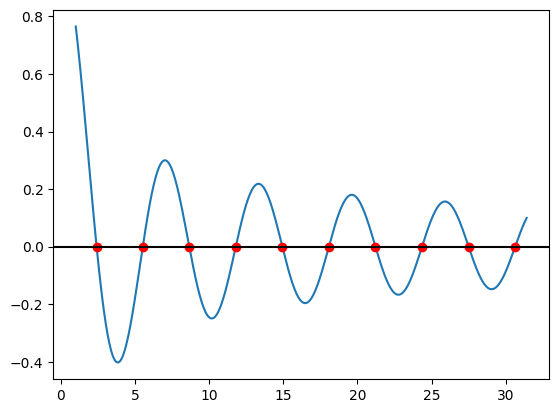
\includegraphics{Include/Images/Thesis/Documentation/NonLinear/Bisect Example 2.png}
    \caption{Bisect Example 2}
    \label{fig:Bisect Example 2}
\end{figure}
}

\subsection{Newton's Method}
Most numerical methods classes use this approach to illustrate the secant method, which is why we built it; nevertheless, it should be noted that according to the method, this is the only one that needs the input of the derivative.
\subsubsection{Examples}
	\paragraph{Example 1}{
\begin{lstlisting}[language=Python]
from BNumMet.NonLinear import newton
fun = lambda x: x**2 - 2
derivative = lambda x: 2 * x
interval = [1, 2]
sol, nIter = newton(fun, derivative, start_point=2, iters = True)
print("Newton's method: x = %f, nIter = %d" % (sol, nIter))
\end{lstlisting}
}
\paragraph{Example 2}{
\begin{lstlisting}[language=Python]
from BNumMet.NonLinear import newton
f = lambda x: sp.jv(0, x)  # Bessel function of the first kind of order 0
derivative = lambda x: sp.jvp(0, x, 1)  # Derivative of the Bessel function
interval = lambda n: [n * np.pi, (n + 1) * np.pi]  # Interval for the n-th zero

zeros = [newton(f, derivative, start_point=interval(n)[0]) for n in range(1, 11)]


x = np.arange(1, 10 * np.pi, np.pi / 50)
y = f(x)
plt.plot(x, y)
plt.plot(zeros, np.zeros(len(zeros)), "ro")
plt.axhline(0, color="k")
plt.title("Zeros of $J_0(x)$ with Newton's method")
plt.xlabel("$x$")
plt.ylabel("$J_0(x)$")
plt.show()
\end{lstlisting}
}
\begin{figure}[H]
    \centering
    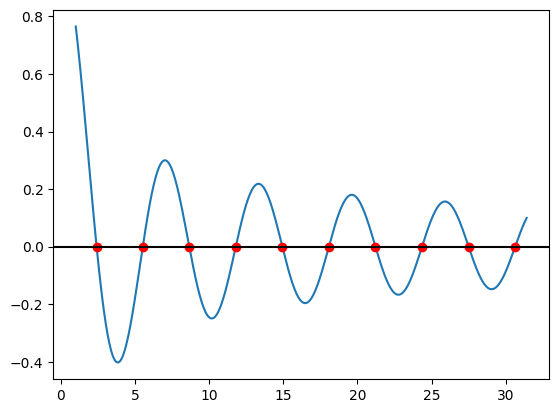
\includegraphics{Include/Images/Thesis/Documentation/NonLinear/Newtons Example 2.png}
    \caption{Newton's Method Example 2}
    \label{fig:Newton's Method Example 2}
\end{figure}


\subsection{Secant Method}
As a continuation of Newton's approach, it is critical to apply the Secant method, which generalizes Newton's method by approximating the derivative and eliminating the necessity for the derivative that Newton's method requires. 
\subsubsection{Examples}
	\paragraph{Example 1}{
\begin{lstlisting}[language=Python]
from BNumMet.NonLinear import secant
fun = lambda x: x**2 - 2
interval = [1, 2]
sol, nIter = secant(fun, interval, iters = True)
print("Secant method: x = %f, nIter = %d" % (sol, nIter))

>> Secant method: x = 1.414214, nIter = 7
\end{lstlisting}
}
\paragraph{Example 2}{
\begin{lstlisting}[language=Python]
f = lambda x: sp.jv(0, x) # Bessel function of the first kind of order 0
interval = lambda n: [n * np.pi, (n + 1) * np.pi] # Interval for the n-th zero

zeros = [ secant(f, interval(n)) for n in range(0, 10)]


x = np.arange(1, 10 * np.pi, np.pi / 50)
y = f(x)
plt.plot(x, y)
plt.plot(zeros, np.zeros(len(zeros)), "ro")
plt.axhline(0, color="k")
plt.show()
\end{lstlisting}
\begin{figure}[H]
    \centering
    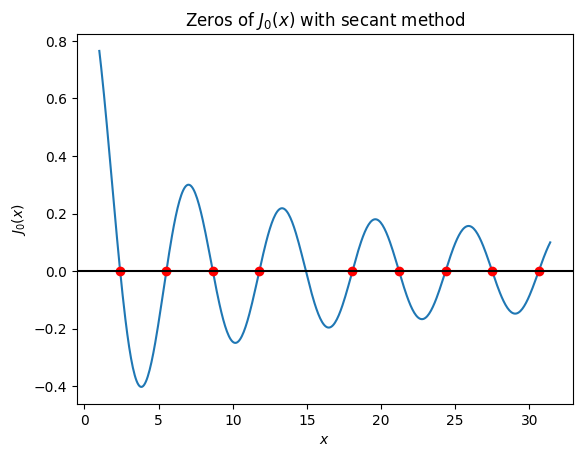
\includegraphics{Include/Images/Thesis/Documentation/NonLinear/Secant Example 2.png}
    \caption{Secant Example 2}
    \label{fig:Secant Example 2}
\end{figure}
}

\subsection{Inverse Quadratic Interpolation (I.Q.I.)}
The aim is to utilize quadratic interpolation to approximate the inverse of f, and further iterations will result in the zero we want. It should be noted that this method is often used as part of another method that we will examine later \cite{10.5555/2553197}, that is why we created it as a standalone to offer students with a glimpse of what the method is about without additional code that may interfere with the learning process.

\subsubsection{Examples}
	\paragraph{Example 1}{
\begin{lstlisting}[language=Python]
from BNumMet.NonLinear import IQI
fun = lambda x: x**2 - 2
points = [1, 1.5 ,2]
sol, nIter = IQI(fun, points, iters = True)
print("IQI method: x = %f, nIter = %d" % (sol, nIter))

>> IQI method: x = 1.414214, nIter = 6
\end{lstlisting}
}
\paragraph{Example 2}{
\begin{lstlisting}[language=Python]
from BNumMet.NonLinear import IQI
f = lambda x: sp.jv(0, x)  # Bessel function of the first kind of order 0
interval = lambda n: [
    n * np.pi,
    (((n + 1) * np.pi) - n * np.pi) / 2,
    (n + 1) * np.pi,
]  # Interval for the n-th zero

zeros = [IQI(f, interval(n)) for n in range(0, 7)]


x = np.arange(1, 10 * np.pi, np.pi / 50)
y = f(x)
plt.plot(x, y)
plt.plot(zeros, np.zeros(len(zeros)), "ro")
plt.axhline(0, color="k")
plt.title("Zeros of $J_0(x)$ with IQI method")
plt.xlabel("$x$")
plt.ylabel("$J_0(x)$")
plt.show()
\end{lstlisting}

\begin{figure}[H]
    \centering
    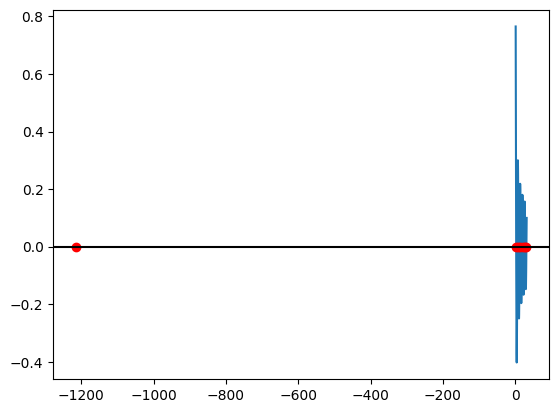
\includegraphics{Include/Images/Thesis/Documentation/NonLinear/IQI Example 2.png}
    \caption{IQI Example 2}
    \label{fig:IQI Example 2}
\end{figure}
}


\subsection{Brent-Dekker's Algorithm}
Brent Dekkers algorithm is one of the methods that combines the previously discussed methods into a method that will improve the number of evaluations a specific method may require while also eliminating some of the caveats that, for example, the secant method has, where there are functions where this latter method does not converge.  It should be noted that this approach was first developed by Dekker, Wiengarten, and their colleagues, only to be modified by Brent to improve convergence. \cite{brent2002algorithms} 

The fundamental idea of Brent-Dekker's Algorithm is to apply the bisection, secant, and if possible the I.Q.I. method, the fundamental criteria of choice is firstly the availability of the application of I.Q.I. which requires three distinct points, after checking that, if it applies I.Q.I is saved, otherwise the secant is saved to then be compared with the bisection algorithm, whichever of the two passes a tolerance criteria given then they will be applied and the next iteration will commence.


In BNumMet, we mostly used Brent's original approach \cite{Press2007} rather than Matlab's for a variety of reasons. One of them is the license under which Matlab allows the code to be used; since our goal was to follow open source initiatives, we needed to use the original one. We also wanted to show students the historical accuracy of the algorithm and present a method that preserves the historical context as well as its current properties. 

In the next paragraph, we will examine the several implementations we discovered, including Matlab's implementation, the original implementation, and Scipy's implementation.

\subsubsection{Analysis of implementations}
The analysis of this package differs from the previous two (linear systems and interpolation packages), where we draw our attention to the syntax and it benefits, in this analysis we will focus on comparing the same method over different plausible implementations that might differ slightly on the code but have a humongous impact on the results of such slight algorithmic differences.

In particular, we will focus on the different implementations the Brentt-Dekker algorithm can have; we will tackle the following:
\begin{enumerate}
    \item Scipy's Brentt Method: The commonly used library for scientific computing has its own implementation of Brent-Dekker's Algorithm. However, the code is not publicly visible. We will discuss how to obtain results without knowing how it works.
    \item Matlab's - Cleve Moller' Implementation: As we discussed, this project has the underlying idea of Cleve Moller's book \cite{doi:10.1137/1.9780898717952}, that is why we have made the translation of this algorithm into Python to properly test it, though it must be noted we will not be using it in our package as a standalone, since we do not own the right to do so.
    \item Original Brent-Dekker's Algorithm: Following the original documentation of Brent \cite{brent2002algorithms} we have translated the procedure given in Chapter 4 of Brent's work into Python.
\end{enumerate}

In this analysis we are interested in how many function evaluation does the algorithm need to find the root, the fundamental reason that we are interested in the number of evaluations is because this types of algorithms do not have an excessive algorithmic complexity, making the evaluation of the function that (most likely) will be nonlinear carry all the computational cost, that is why we need to find the number of evaluations. However, we are unable to look at Scipy's code to tamper with it to obtain our desired result, to properly proceed I want to digress from the discussion at hand and focus on how we can find the number of function evaluations without the need of having the actual implementation.

\paragraph{Finding function evaluations without external code} As a thought experiment, imagine you have a machine that is protected so as not to be opened or tampered with, this machine can only take in a function $f(x)$ and outputs its zero (for arguments sake, suppose it can be done without any problems), this machine does not output how many times did it use the function to calculate or has a small light that shows how it is processing. We can only input functions and have as an output the location of the zero. 




\tikzset{every picture/.style={line width=0.75pt}} %set default line width to 0.75pt        

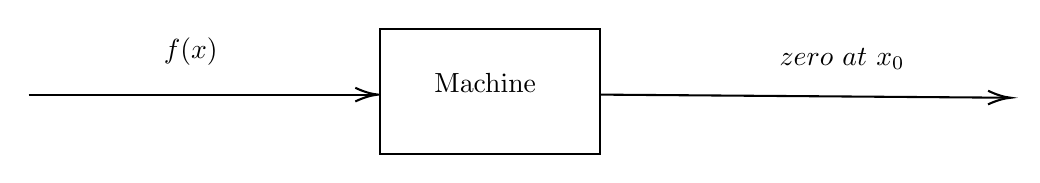
\begin{tikzpicture}[x=0.75pt,y=0.75pt,yscale=-1,xscale=1]
%uncomment if require: \path (0,141); %set diagram left start at 0, and has height of 141

%Straight Lines [id:da07216189034981646] 
\draw    (95,71.28) -- (261.29,71.28) ;
\draw [shift={(263.29,71.28)}, rotate = 180] [color={rgb, 255:red, 0; green, 0; blue, 0 }  ][line width=0.75]    (10.93,-3.29) .. controls (6.95,-1.4) and (3.31,-0.3) .. (0,0) .. controls (3.31,0.3) and (6.95,1.4) .. (10.93,3.29)   ;
%Shape: Rectangle [id:dp6037570291001613] 
\draw  [fill={rgb, 255:red, 255; green, 255; blue, 255 }  ,fill opacity=1 ] (264.3,39.53) -- (370.12,39.53) -- (370.12,100) -- (264.3,100) -- cycle ;
%Straight Lines [id:da284111323999086] 
\draw    (370.62,71.28) -- (566.14,72.78) ;
\draw [shift={(568.14,72.79)}, rotate = 180.44] [color={rgb, 255:red, 0; green, 0; blue, 0 }  ][line width=0.75]    (10.93,-3.29) .. controls (6.95,-1.4) and (3.31,-0.3) .. (0,0) .. controls (3.31,0.3) and (6.95,1.4) .. (10.93,3.29)   ;

% Text Node
\draw (158.6,42.52) node [anchor=north west][inner sep=0.75pt]    {$f( x)$};
% Text Node
\draw (455.28,47.56) node [anchor=north west][inner sep=0.75pt]    {$zero\ at\ x_{0}$};
% Text Node
\draw (289,59.67) node [anchor=north west][inner sep=0.75pt]   [align=left] {Machine};


\end{tikzpicture}



One could argue why not create a function that counts the evaluation every time it is invoked; something of this sort will reassemble: 
\begin{lstlisting}
FUNCTION 
    IN : x
    PERFORM : 
        evaluations +=1
    OUT : f(x)
\end{lstlisting}

But most programming languages lack the ability to auto-initialise the value, and even if initialised it must be done inside the function itself which will be reset every function evaluation.

Imagine we can create a function (think of if as a piece of hardware) that can safely be input to our machine and still have our expected zero, but we  can create one 'invisible' cable that is connected to a light outside the machine, and every time it evaluates the function, the light is turned on (or in this case a counter is updated). To do such thing, we must draw our attention to Global Variables, variables that are within the reach of the entire execution of a program and can be edited and accessed anywhere in the code. 

This idea will look like 
\begin{lstlisting}
global evaluations = 0
FUNCTION 
    IN : x
    PERFORM : 
        evaluations +=1
    OUT : f(x)
\end{lstlisting}


Once this link is created, we only need to reset the counter every time we input a new function, and we will obtain the evaluations they did of the function.



\tikzset{every picture/.style={line width=0.75pt}} %set default line width to 0.75pt        

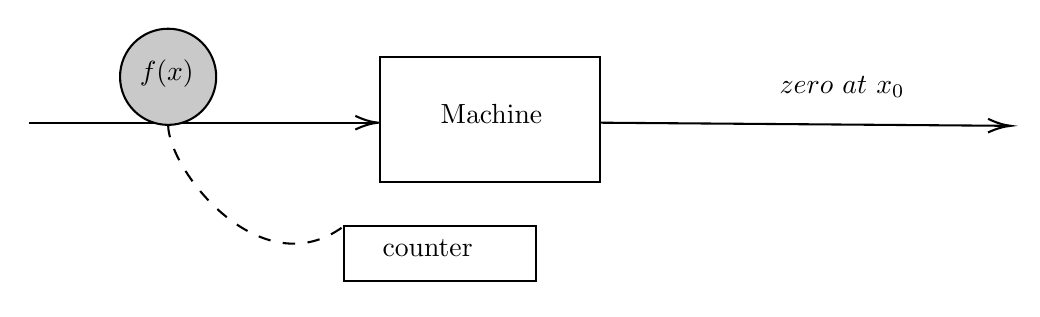
\begin{tikzpicture}[x=0.75pt,y=0.75pt,yscale=-1,xscale=1]
%uncomment if require: \path (0,190); %set diagram left start at 0, and has height of 190

%Straight Lines [id:da8004978280594872] 
\draw    (99,89.28) -- (265.29,89.28) ;
\draw [shift={(267.29,89.28)}, rotate = 180] [color={rgb, 255:red, 0; green, 0; blue, 0 }  ][line width=0.75]    (10.93,-3.29) .. controls (6.95,-1.4) and (3.31,-0.3) .. (0,0) .. controls (3.31,0.3) and (6.95,1.4) .. (10.93,3.29)   ;
%Shape: Rectangle [id:dp04043727048803203] 
\draw  [fill={rgb, 255:red, 255; green, 255; blue, 255 }  ,fill opacity=1 ] (268.3,57.53) -- (374.12,57.53) -- (374.12,118) -- (268.3,118) -- cycle ;
%Straight Lines [id:da458025777694687] 
\draw    (374.62,89.28) -- (570.14,90.78) ;
\draw [shift={(572.14,90.79)}, rotate = 180.44] [color={rgb, 255:red, 0; green, 0; blue, 0 }  ][line width=0.75]    (10.93,-3.29) .. controls (6.95,-1.4) and (3.31,-0.3) .. (0,0) .. controls (3.31,0.3) and (6.95,1.4) .. (10.93,3.29)   ;
%Flowchart: Connector [id:dp3688737316817359] 
\draw  [fill={rgb, 255:red, 201; green, 201; blue, 201 }  ,fill opacity=1 ] (143,67.17) .. controls (143,54.37) and (153.37,44) .. (166.17,44) .. controls (178.96,44) and (189.33,54.37) .. (189.33,67.17) .. controls (189.33,79.96) and (178.96,90.33) .. (166.17,90.33) .. controls (153.37,90.33) and (143,79.96) .. (143,67.17) -- cycle ;
%Curve Lines [id:da6747445781275441] 
\draw  [dash pattern={on 4.5pt off 4.5pt}]  (166.17,90.33) .. controls (166.33,112.33) and (211,169) .. (251,139) ;
%Shape: Rectangle [id:dp15460904797277109] 
\draw  [fill={rgb, 255:red, 255; green, 255; blue, 255 }  ,fill opacity=1 ] (251,139) -- (343.33,139) -- (343.33,165.33) -- (251,165.33) -- cycle ;

% Text Node
\draw (459.28,65.56) node [anchor=north west][inner sep=0.75pt]    {$zero\ at\ x_{0}$};
% Text Node
\draw (151,57.4) node [anchor=north west][inner sep=0.75pt]    {$f( x)$};
% Text Node
\draw (268,144) node [anchor=north west][inner sep=0.75pt]   [align=left] {counter};
% Text Node
\draw (296,78.67) node [anchor=north west][inner sep=0.75pt]   [align=left] {Machine};

\end{tikzpicture}

\paragraph{Results}
To test it we will implement the thought experiment in code and proceed in the following manner, we will create a function $f(x) = (x-a)\cdot x^{i}$, where $a$ will be either $1$ or $0.1$, a number that can be written in floating-point expression and one that cannot, the $i$ will be the exponent of the function which will take odd values. We will run the 3 aforementioned methods once (since in this case the algorithms are purely deterministic, as they do not rely on time) for different interval widths starting at $0.8$ and ending in $1.1+j$ where j will be increasing from 1 to 10000 in step sizes of 1. Using in all the methods the same input tolerance.

Our goal with this test will be firstly to prove the effectiveness of the original algorithm and the implementation in python with respect to the other two, as well as, observing if we have an algorithmic advantage or not with these aforementioned methods.

We will then take the number of evaluations and the value of x at where the zero is found in order to measure the relative error.

\subparagraph{For $a=1$}
As we can observe in the first plot of [fig \ref{fig:NonLinear 3 method Results for a=1 same tolerance}] Scipy's implementation of Brent-Dekker's Algorithm is the worst in term of number of evaluations, and Matlab's has almost everywhere a similar behaviour in number of evaluations. Looking at the second plot, we see that even though BNumMet's implementation was better in terms of evaluations, it is the worst in terms of relative error, and Matlab's is similar to Scipy's but slightly worst.

One question rises from here: will BNumMets implementation improve - in terms of having a lower number of function evaluations - if we reduce the tolerance, at the risk of number of evaluations - but as seen, we still have room for tweaking. In fact, we can improve the relative error of BNumMets by decreasing the tolerance and still have an advantage over Scipy's implementation almost everywhere [fig \ref{fig:NonLinear 3 method Results for a=1 BNumMet smaller tolerance}]

This results proves that the original implementation of Brent-Dekker is better than Scipy's, because at a lower number of function evaluations we achieve a better relative error. 

\subparagraph{For $a=0.1$}
The same discussion of $a=1$ remains valid to the case $a=0.1$, it must be noted that in this case the plots show a extravagant behaviour, with the number of evaluations, at certain points, the evaluations remain the same regardless of the interval size. On the first plot [fig \ref{fig:NonLinear 3 method Results for a=0.1 same tolerance}] we observe that BNumMet takes the leading position while on the second plot, there remains a high relative error but closer to Matlab's on the overall scheme.

Incrementing the input tolerance to BNumMet's implementation, we observe [fig \ref{fig:NonLinear 3 method Results for a=0.1 BNumMet smaller tolerance}] that not only does BNumMet's implementation offer a lower number of function evaluations but also it provides a better relative error in comparison to Scipy's implementation.

All in all, the decision to implement the original Brent-Dekker was a good choice; not only does it preserve the historical algorithm but also improves on the well-known library of Scipy.

\begin{sidewaysfigure}[htbp]
    \centering
    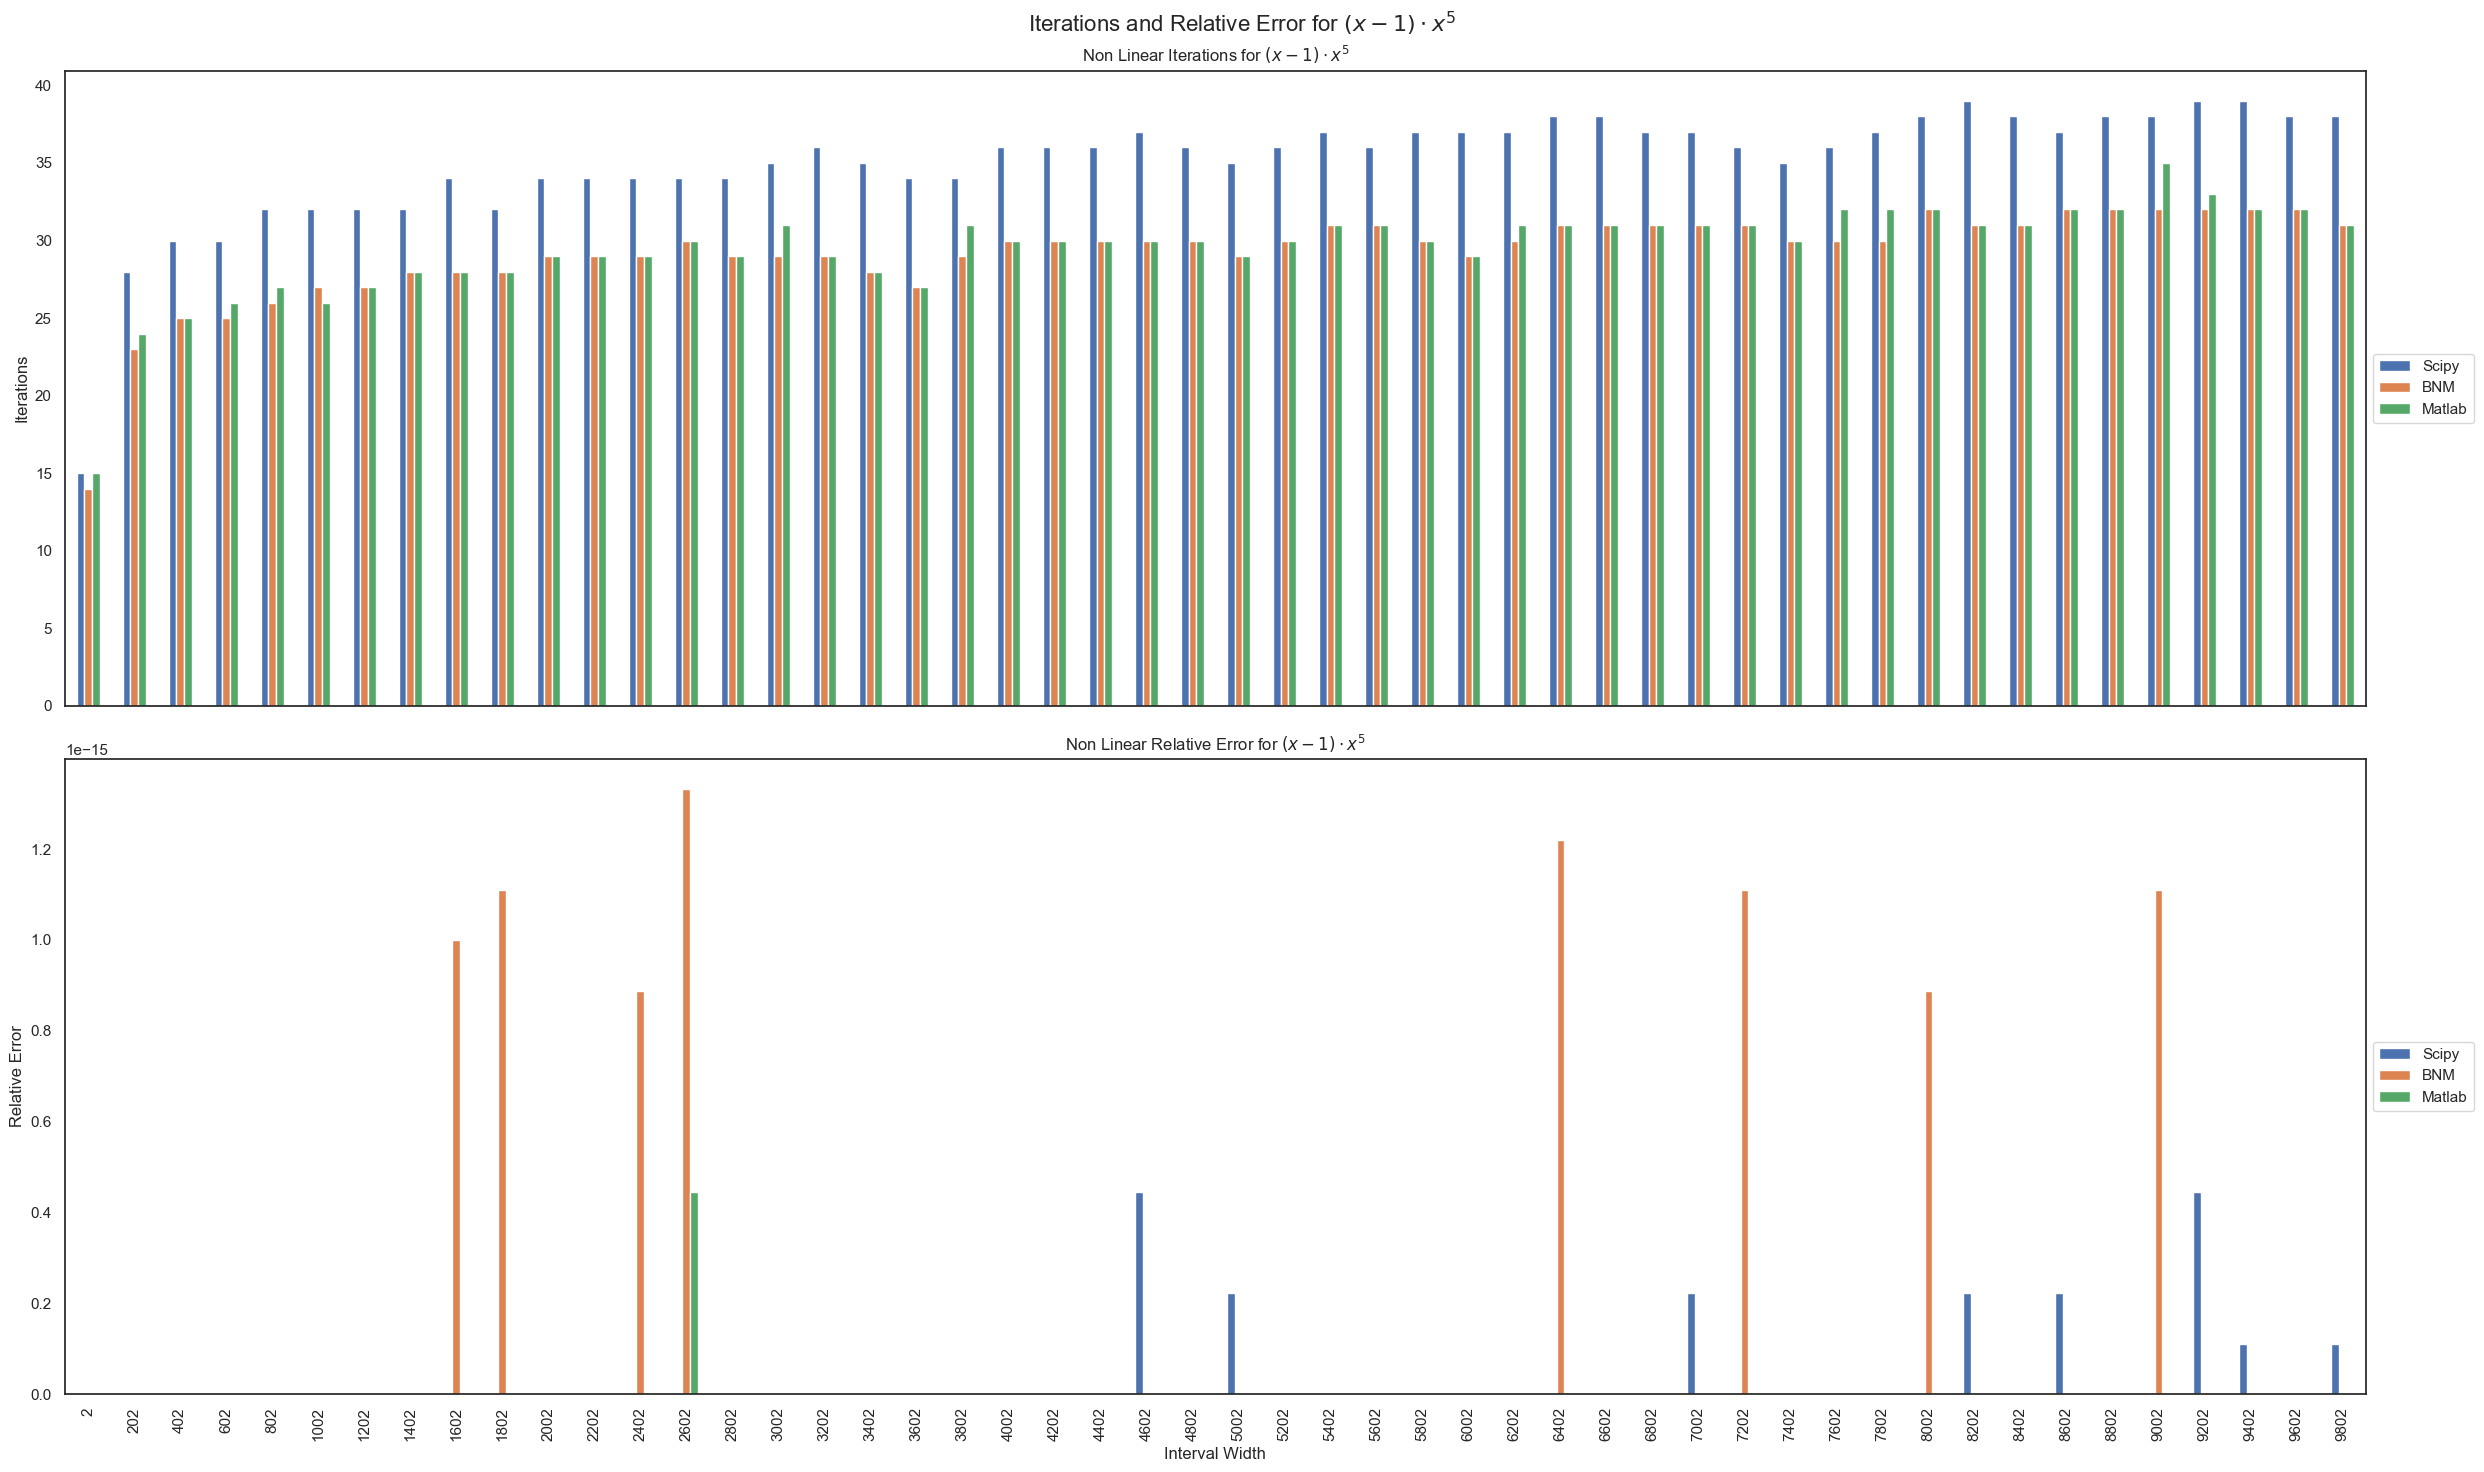
\includegraphics[width=\textwidth]{Include/Images/Thesis/Analysis of Solutions/NonLinear AS/NonLinear 3 method Results a-1.png}
    \caption{NonLinear 3 method Results for $a=1$ same tolerance}
    \label{fig:NonLinear 3 method Results for a=1 same tolerance}
\end{sidewaysfigure}

\begin{sidewaysfigure}[htbp]
    \centering
    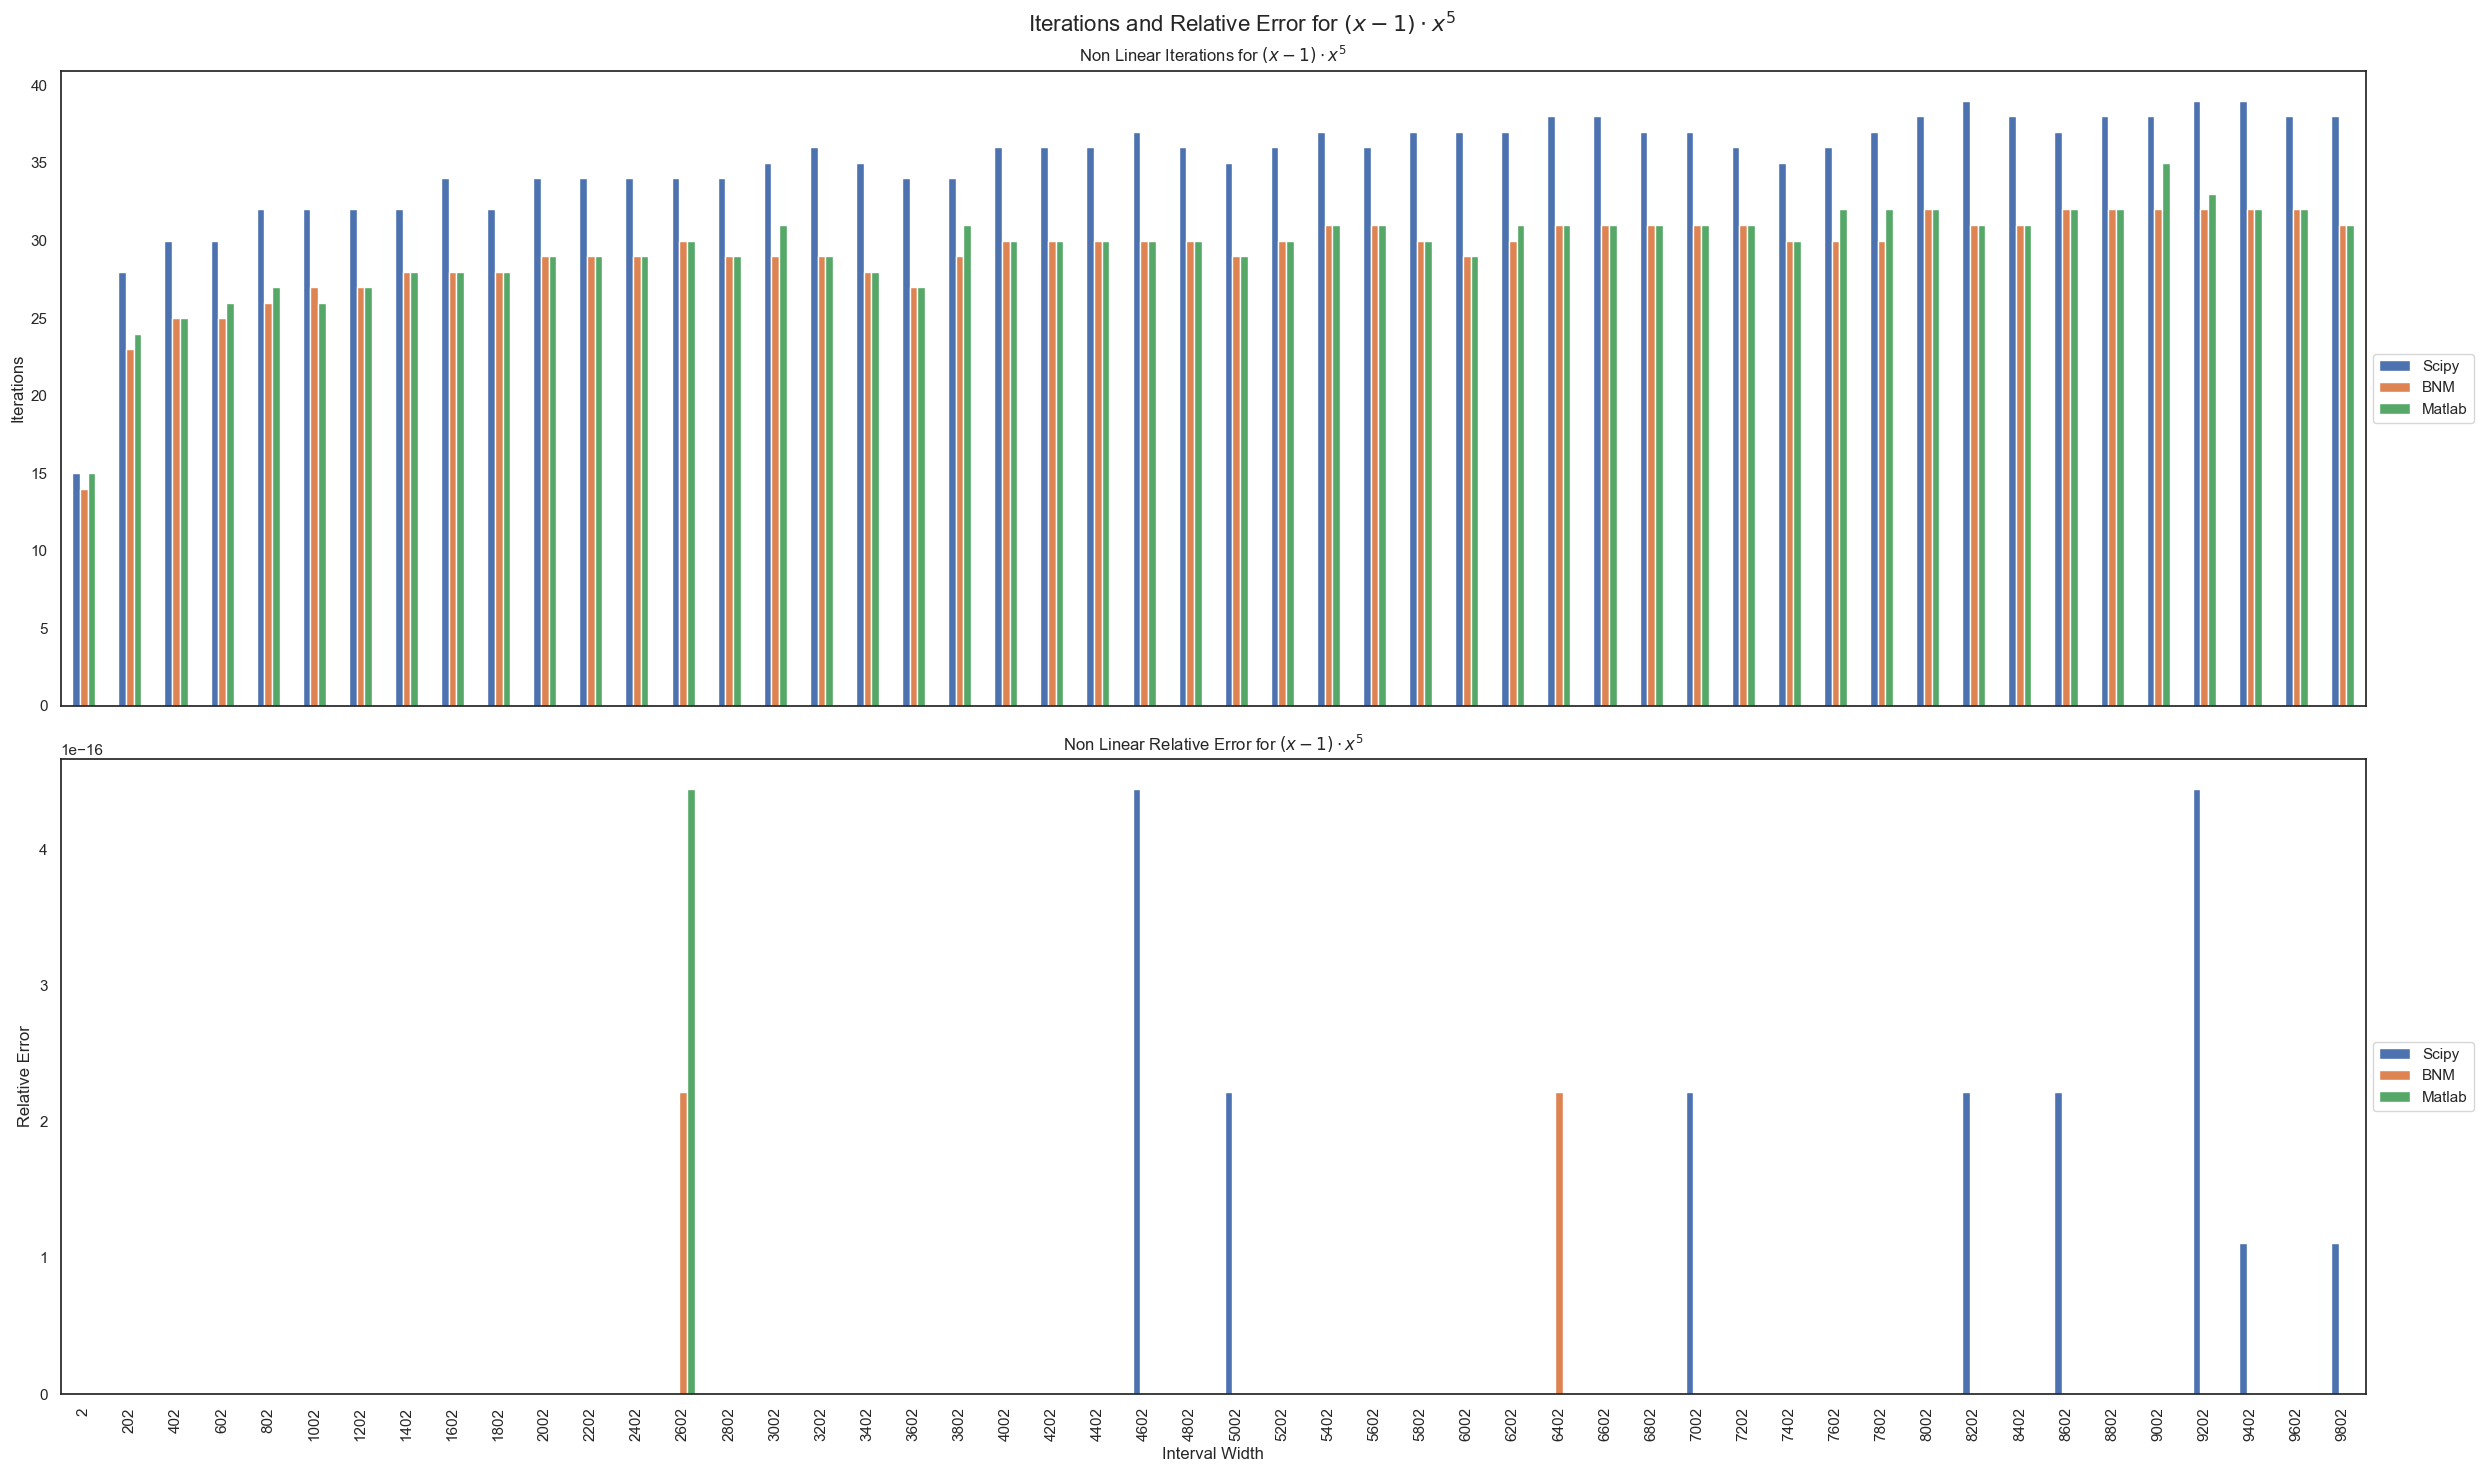
\includegraphics[width=\textwidth]{Include/Images/Thesis/Analysis of Solutions/NonLinear AS/NonLinear 3 method Results Small Tol Bnum a-1.png}
    \caption{NonLinear 3 method Results for $a=1$ BNumMet smaller tolerance}
    \label{fig:NonLinear 3 method Results for a=1 BNumMet smaller tolerance}
\end{sidewaysfigure}

\begin{sidewaysfigure}[htbp]
    \centering
    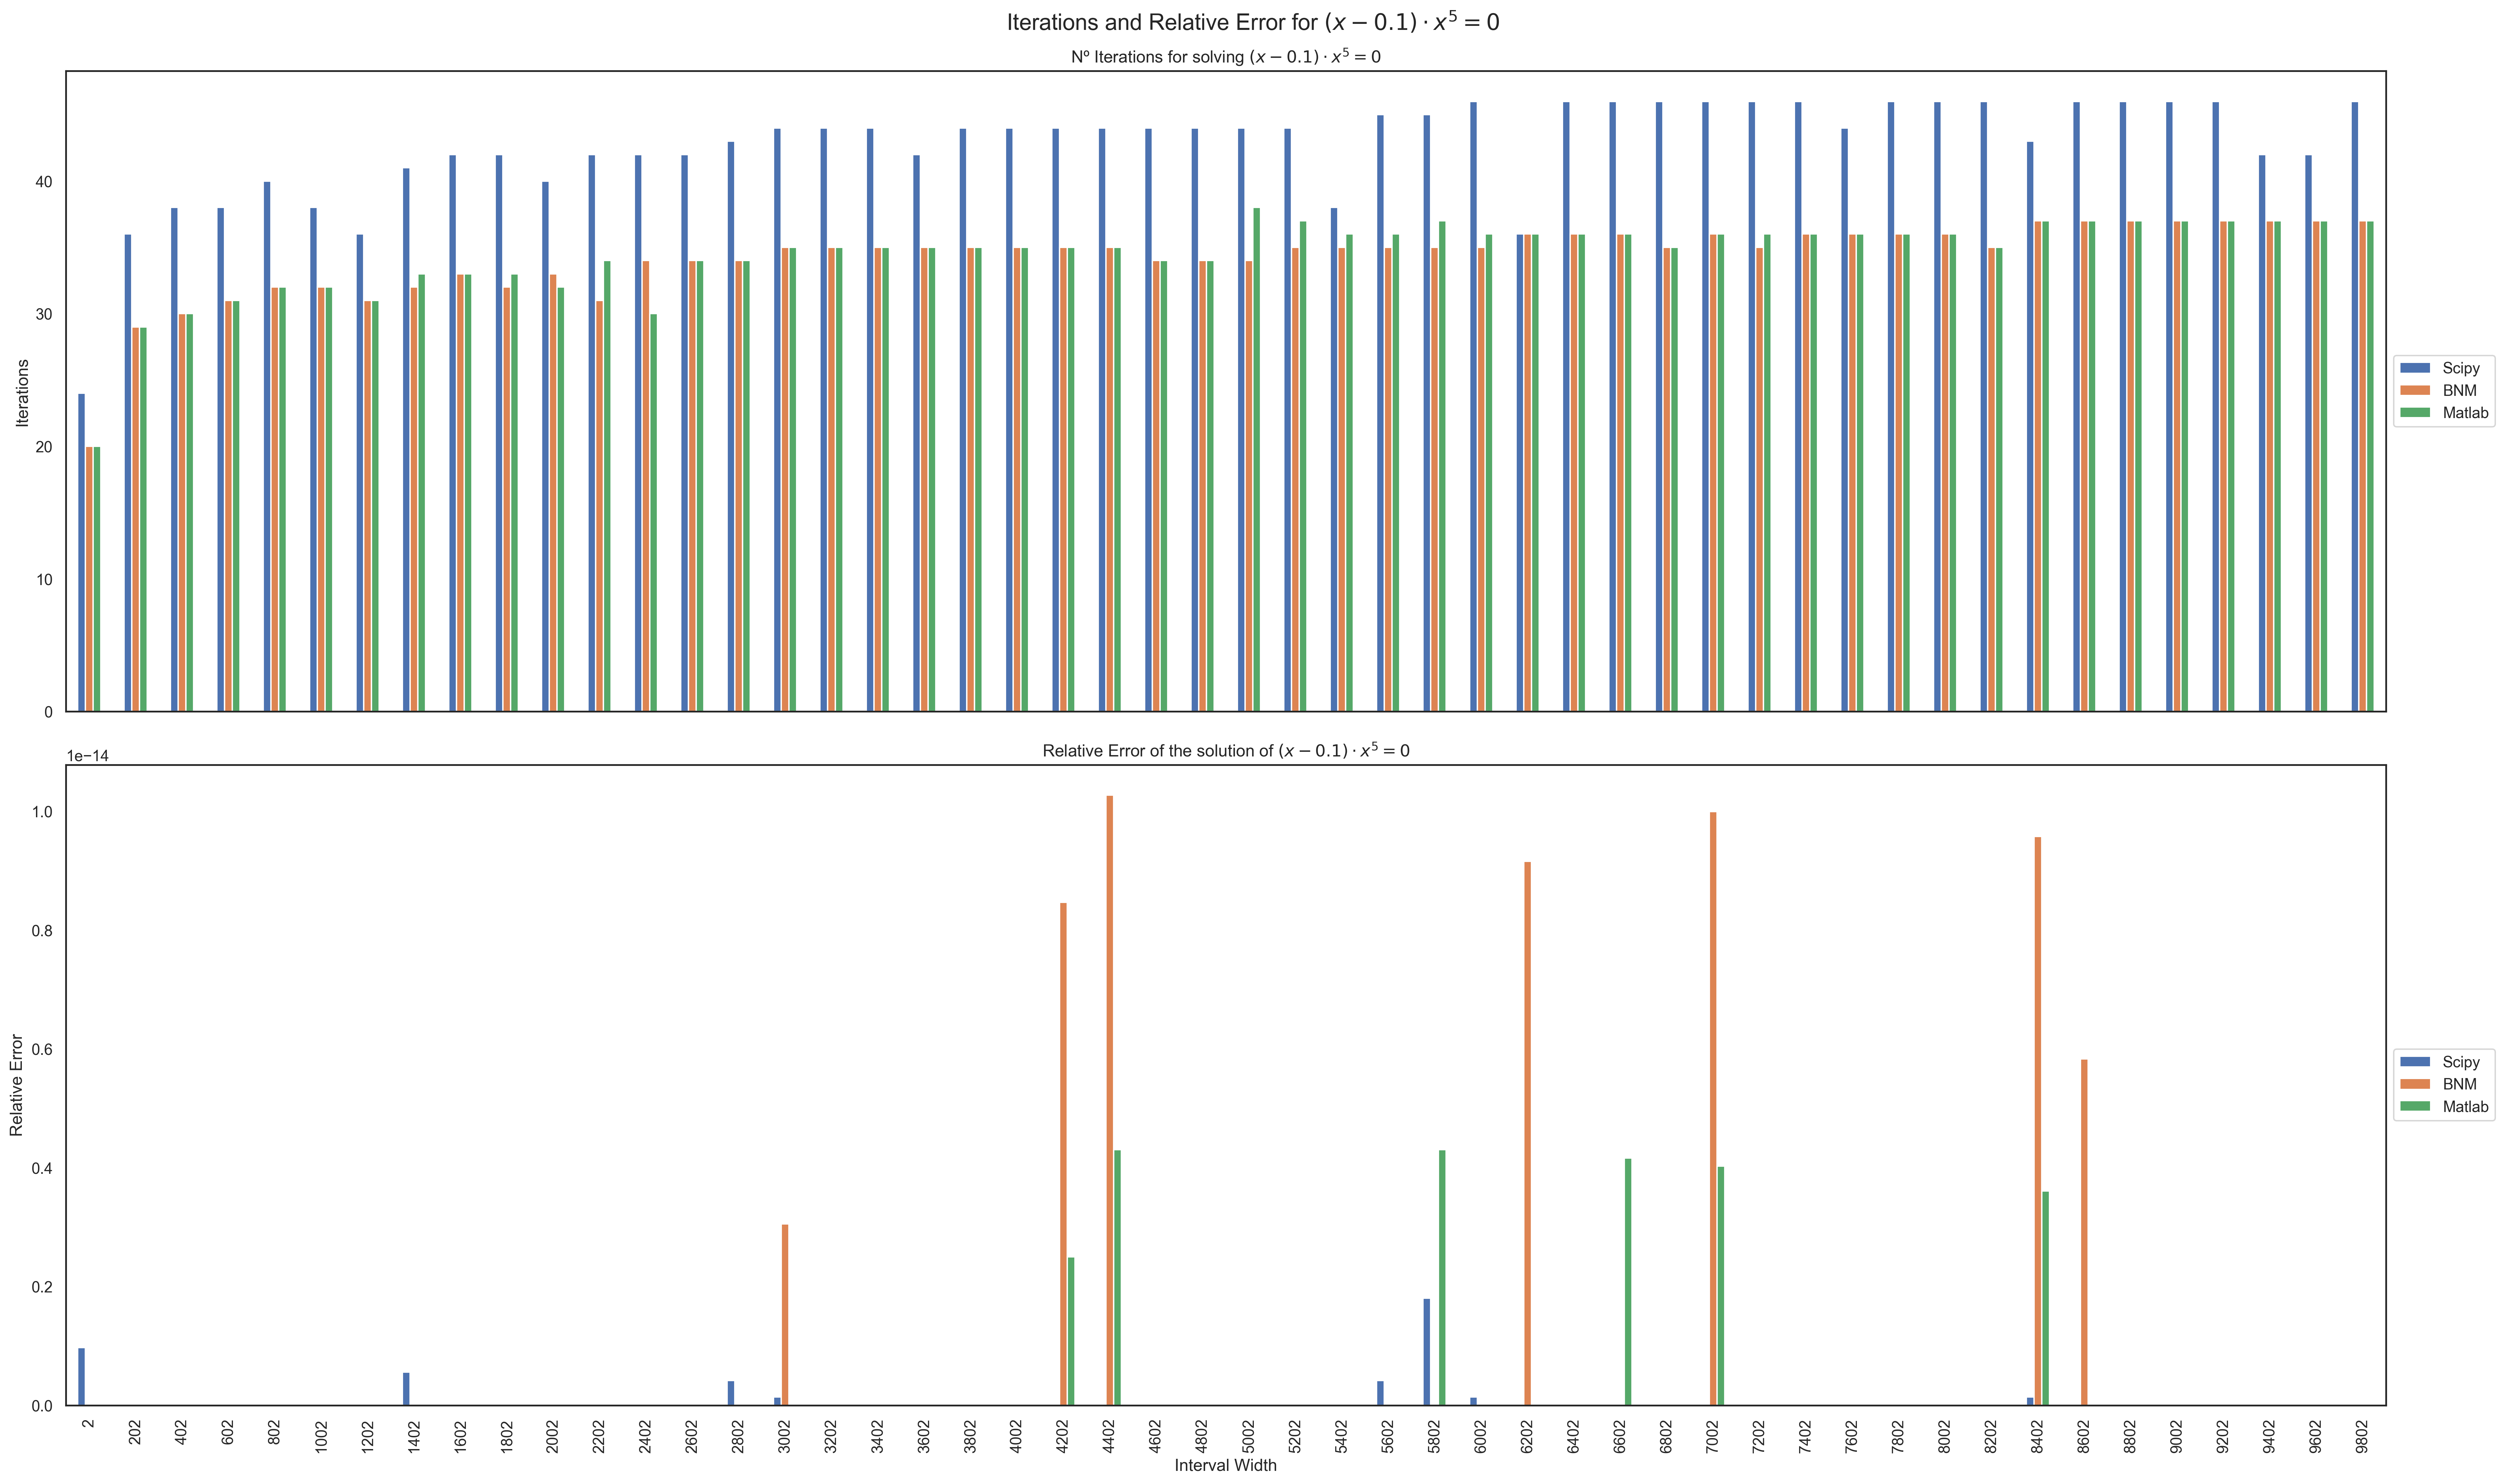
\includegraphics[width=\textwidth]{Include/Images/Thesis/Analysis of Solutions/NonLinear AS/NonLinear 3 method Results a-0.1.png}
    \caption{NonLinear 3 method Results for $a=0.1$ same tolerance}
    \label{fig:NonLinear 3 method Results for a=0.1 same tolerance}
\end{sidewaysfigure}

\begin{sidewaysfigure}[htbp]
    \centering
    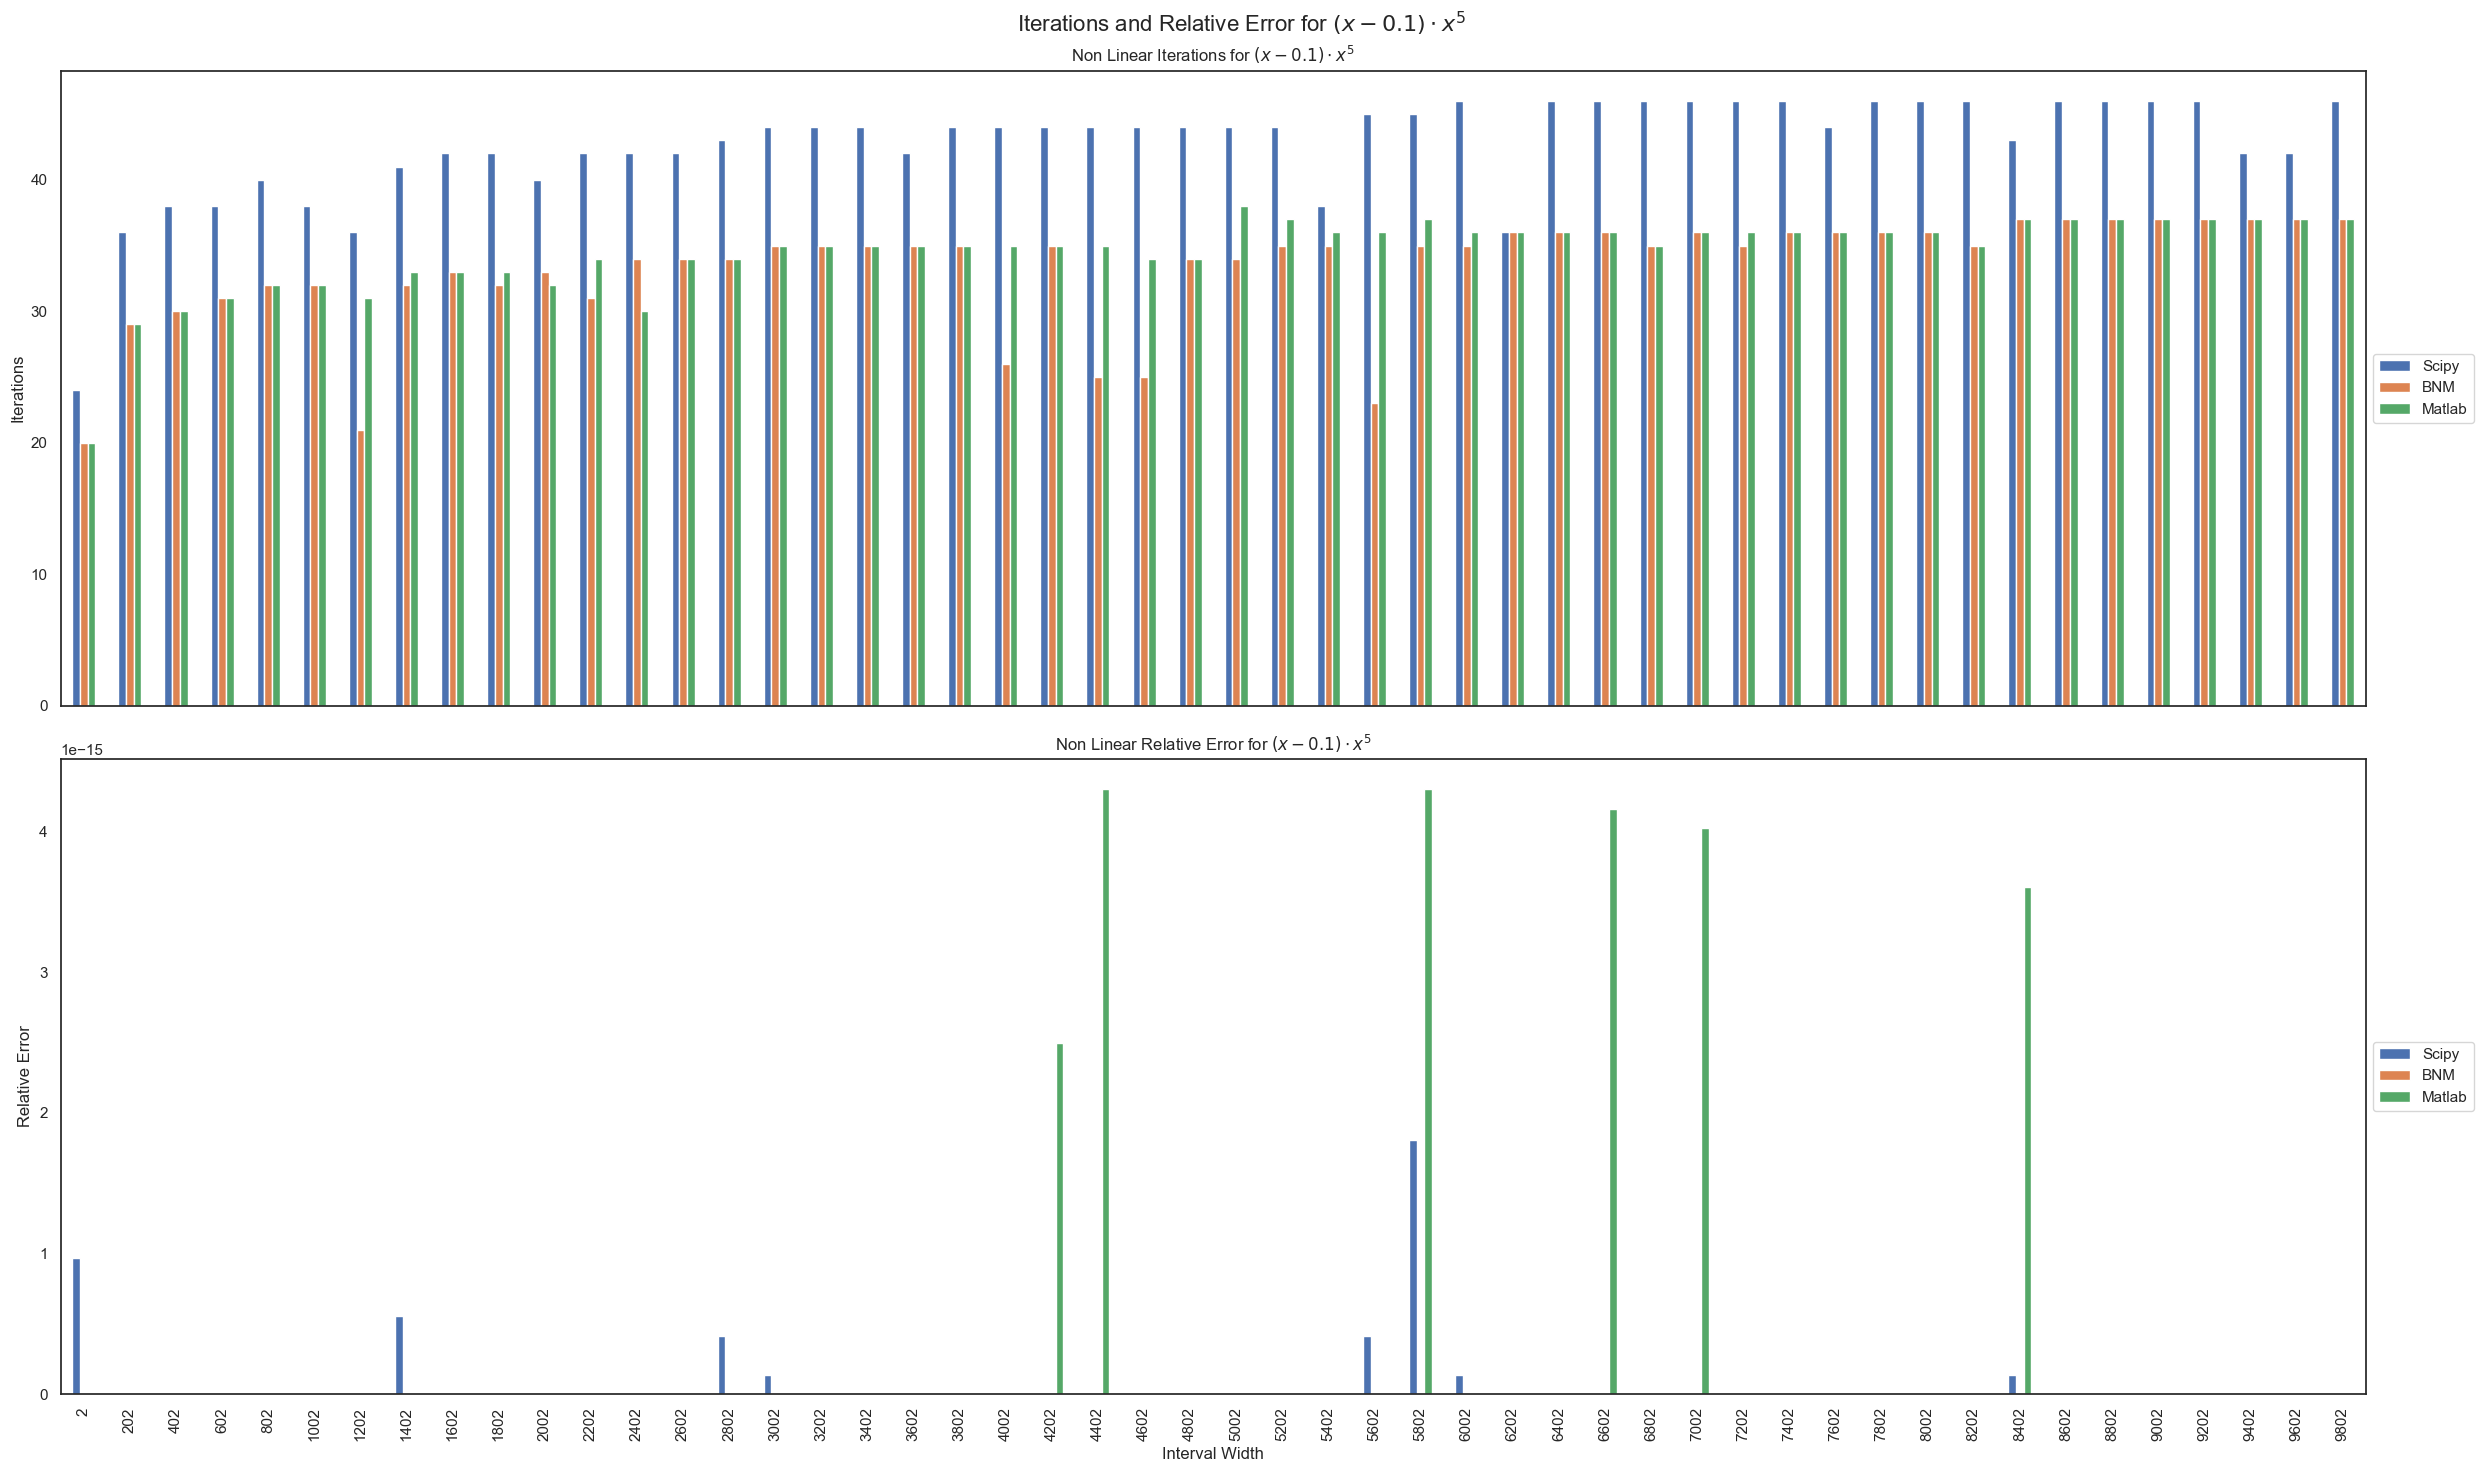
\includegraphics[width=\textwidth]{Include/Images/Thesis/Analysis of Solutions/NonLinear AS/NonLinear 3 method Results Small Tol Bnum a-0.1.png}
    \caption{NonLinear 3 method Results for $a=0.1$ BNumMet smaller tolerance}
    \label{fig:NonLinear 3 method Results for a=0.1 BNumMet smaller tolerance}
\end{sidewaysfigure}


\subsubsection{Examples}
	\paragraph{Example 1}{
\begin{lstlisting}[language=Python]
from BNumMet.NonLinear import zBrentDekker
fun = lambda x: x**2 - 2
interval = [1, 2]
sol, nIter = zBrentDekker(fun, interval, iters = True)
print("Brent-Dekker method: x = %f, nIter = %d" % (sol, nIter))

>> Brent-Dekker method: x = 1.414214, nIter = 7
\end{lstlisting}
}
\paragraph{Example 2}{
\begin{lstlisting}[language=Python]
f = lambda x: sp.jv(0, x) # Bessel function of the first kind of order 0
interval = lambda n: [n * np.pi, (n + 1) * np.pi] # Interval for the n-th zero

zeros = [ zBrentDekker(f, interval(n)) for n in range(0, 10)]


x = np.arange(1, 10 * np.pi, np.pi / 50)
y = f(x)
plt.plot(x, y)
plt.plot(zeros, np.zeros(len(zeros)), "ro")
plt.axhline(0, color="k")
plt.show()
\end{lstlisting}
\begin{figure}[H]
    \centering
    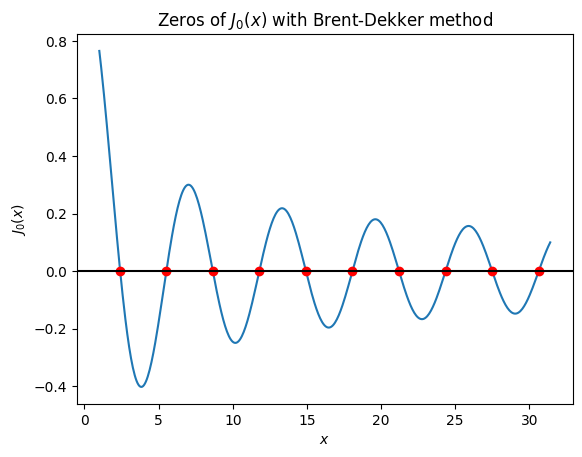
\includegraphics{Include/Images/Thesis/Documentation/NonLinear/Brentt-Dekker Example 2.png}
    \caption{Brentt-Dekker Example 2}
    \label{fig:Brentt-Dekker Example 2}
\end{figure}
}
